\section{Задание 3. Системы линейных алгебраических уравнений (СЛАУ).}

\textbf{Условие.}\\
Даны две системы линейных алгебраических уравнений:
Решите задачу по плану:
\begin{enumerate}
    \item Найдите базисный минор (не только порядок!) основной матрицы каждой системы.
    \item Найдите ранг расширенной матрицы системы. Сделайте вывод о совместности и
    определенности систем на основании теоремы Кронекера-Капелли и следствий из нее.
    \item Совместную определенную систему (если она есть) решите методом обратной матрицы.
    \item Для несовместной или совместной неопределенной системы:
    \begin{enumerate}
        \item Запишите соответствующую однородную систему. Найдите базис подпространства,
        заданного этой системой. Изобразите подпространство решений на графике, как
        линейную оболочку базисных векторов.
        \item Найдите общее решение неоднородной системы (если она совместна), изобразите его на
        том же графике.
    \end{enumerate}
\end{enumerate}

\begin{enumerate}
    \item $\begin{cases}
              2x - y + z = 2 \\
              3x + 2y + 2z = -2 \\
              x - 2y + z = 1
    \end{cases}$
    \item $\begin{cases}
              x + 2y + 3z = 2 \\
              x + y + z = -1 \\
              3x + y - z = 3
    \end{cases}$
\end{enumerate}
\vspace{10mm}
\noindent\textbf{Решение.}\\
\begin{enumerate}
    \item $\begin{cases}
              2x - y + z = 2 \\
              3x + 2y + 2z = -2 \\
              x - 2y + z = 1
    \end{cases}$

    Пусть $A = \begin{pmatrix}2 & -1 & 1\\ 3 & 2 & 2 \\ 1 & -2 & 1\end{pmatrix}$; $B = \begin{pmatrix}2 \\ -2 \\ 1\end{pmatrix}$

    $(A|B) = \begin{pmatrix}2 & -1 & 1\\ 3 & 2 & 2 \\ 1 & -2 & 1\end{pmatrix}\begin{pmatrix}2 \\ -2 \\ 1\end{pmatrix}
    \quad\sim\quad
    \begin{pmatrix}2 & -1 & 1\\ 0 & 8 & -1 \\ 1 & -2 & 1\end{pmatrix}\begin{pmatrix}2 \\ -5 \\ 1\end{pmatrix}
    \quad\sim\quad
    \begin{pmatrix}2 & -1 & 1\\ 0 & 8 & -1 \\ 0 & -\frac{3}{2} & \frac{1}{2}\end{pmatrix}\begin{pmatrix}2 \\ -5 \\ 0\end{pmatrix}
    \quad\sim\quad
    \begin{pmatrix}2 & -1 & 1\\ 0 & 8 & -1 \\ 0 & 0 & \frac{5}{16}\end{pmatrix}\begin{pmatrix}2 \\ -5 \\ -\frac{15}{16}\end{pmatrix}$

    Как видно, ступенчатый вид основной и расширенной матриц не имеет нулевых строчек,
    следовательно, $rang(A) = rang(A|B) = 3$, что по теореме Кронекера-Капелли значит, что СЛАУ совместна и определена.

    Исходная матрица $A = \begin{pmatrix}2 & -1 & 1\\ 3 & 2 & 2 \\ 1 & -2 & 1\end{pmatrix}$ является базисным минором

    $\displaystyle \begin{cases}
         2x - y + z &= 2 \\
             8y - z &= -5 \\
      \frac{5z}{16} &= -\frac{15}{16}
    \end{cases}\\
    \begin{cases}
        z &= -3 \\
        y &= -1 \\
        x &= 2
    \end{cases}$

    \textit{Ответ}: $(2; -1; -3)$.
    \vspace{10mm}

    \item $\begin{cases}
              x + 2y + 3z = 2 \\
              x + y + z = -1 \\
              3x + y - z = 3
    \end{cases}$

    Пусть $A = \begin{pmatrix}1 & 2 & 3\\ 1 & 1 & 1 \\ 3 & 1 & -1\end{pmatrix}$; $B = \begin{pmatrix}2 \\ -1 \\ 3\end{pmatrix}$

    $(A|B) = \begin{pmatrix}1 & 2 & 3\\ 1 & 1 & 1 \\ 3 & 1 & -1\end{pmatrix}\begin{pmatrix}2 \\ -1 \\ 3\end{pmatrix}
    \quad\sim\quad
    \begin{pmatrix}1 & 2 & 3\\ 0 & -1 & -2 \\ 3 & 1 & -1\end{pmatrix}\begin{pmatrix}2 \\ -3 \\ 3\end{pmatrix}
    \quad\sim\quad
    \begin{pmatrix}1 & 2 & 3\\ 0 & -1 & -2 \\ 0 & -5 & -10\end{pmatrix}\begin{pmatrix}2 \\ -3 \\ -3\end{pmatrix}
    \quad\sim\quad
    \begin{pmatrix}1 & 2 & 3\\ 0 & -1 & -2 \\ 0 & 0 & 0\end{pmatrix}\begin{pmatrix}2 \\ -3 \\ 12\end{pmatrix}$

    Как видно, ступенчатый вид основной матрицы имеет нулевую строчку, а значение в той же строчке матрицы $B$ не равна нулю,
    следовательно, $rang(A) = 2 \neq rang(A|B) = 3$, значит, что система не имеет решений.

    В этом случае, базисным минором будет $\begin{pmatrix}1 & 2\\ 0 & -1\end{pmatrix}$

    Соответствующая однородная система:

    $\begin{cases}
              x + 2y + 3z &= 0 \\
              x + y + z &= 0 \\
              3x + y - z &= 0
    \end{cases} \Longrightarrow
    \begin{pmatrix}1 & 2 & 3\\ 0 & -1 & -2 \\ 0 & 0 & 0\end{pmatrix}\begin{pmatrix}0 \\ 0 \\ 0\end{pmatrix} \Longrightarrow
    \begin{cases}
              x + 2y + 3z &= 0 \\
              -y + -2z &= 0
    \end{cases}  \Longrightarrow
    \begin{cases}
              x &= z \\
              y &= -2z
    \end{cases}$

    Фундаментальной системой решений для этой системы является $(z; -2z; z) = C_1\begin{pmatrix}1 \\ -2 \\ 1\end{pmatrix} \implies$
    размерность подпространства решений - 1, базисом подпространства в таком случае будет $\begin{pmatrix}1 \\ -2 \\ 1\end{pmatrix}$

    \begin{figure}
        \centering
        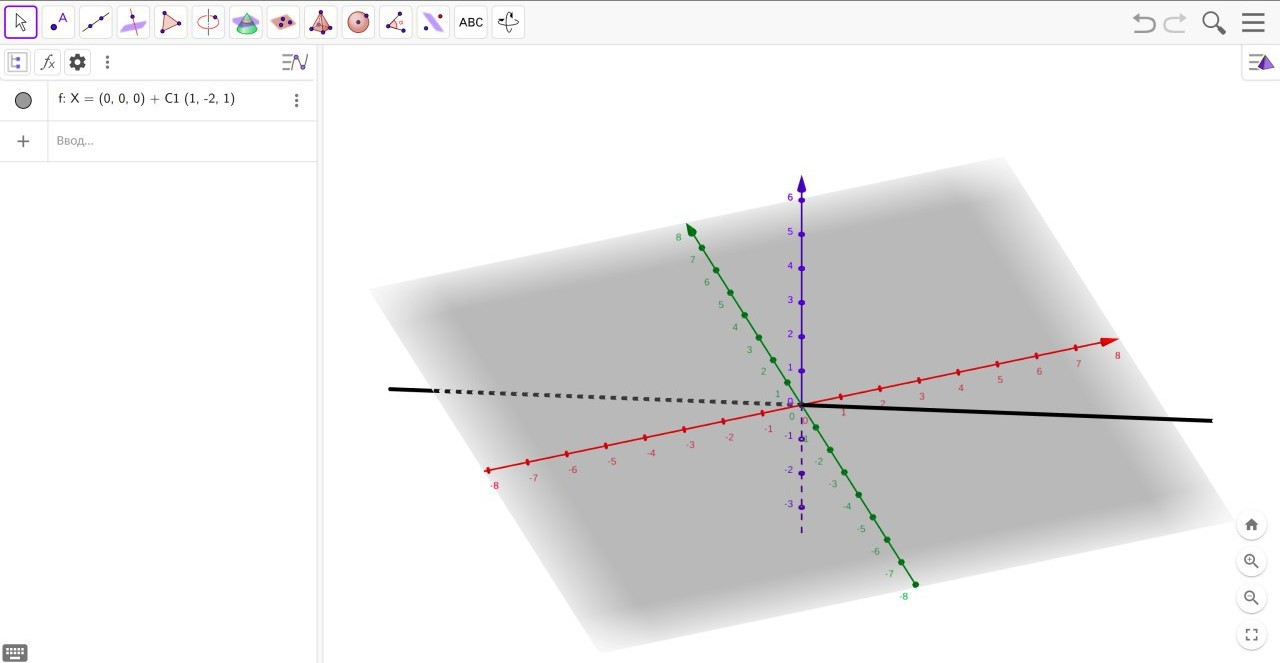
\includegraphics[width=500pt]{images/3b1}
        \caption{График подпространства из пункта (2)}
        \label{fig:}
    \end{figure}

    \textit{Ответ}: общее решение - $C_1\begin{pmatrix}1 \\ -2 \\ 1\end{pmatrix}$.

\end{enumerate}

\clearpage
